\documentclass[10px]{article}
\usepackage{graphicx} % Required for inserting images
\usepackage[english,russian]{babel}
\usepackage{cmap}
\usepackage{array}

\usepackage{cellspace, graphicx, makecell}
%\DeclareGraphicsExtensions{.pdf,.png,.jpg}
\usepackage[left=2cm,right=2cm,
    top=2cm,bottom=2cm]{geometry}
    
\title{Лабораторная работа 1.2.3 \\ Исследование вынужденной регулярной прецессии гироскопа}
\author{Матвей Галицын \\ Б01-411}
\date{November 11, 2024}

\begin{document}
\maketitle

\section{Аннотация}
\indentВ работе измеряется момент инерции ряда тел и сравниваются результаты с расчетами по теоретическим формулам, проверяются аддитивности моментов инерции и справедливости формулы Гюйгенса-Штейнера.

\section{Теоретические сведения}
Возьмем трифилярный подвес. \\
\begin{minipage}[h]{0.6\linewidth}
Уравнение сохранении энергии при крутильных колебаниях можно записать следующим образом:
\begin{center}
    $\frac{I {\dot{\phi}}^2}{2} + mg(z_0 - z) = E$,
\end{center}
где I - момент инерции платформы вместе с исследуемым телом, m - масса платформы с телом, $\phi$ - угол поворота платформы от положения равновесия системы, $z_0$ - координата по вертикали центра нижней платформы $O^\prime$ при равновесии ($\phi$ = 0), $z$ - координата той же точки при некотором угле $\phi$.\\
Так как при по повороте $C^\prime$ в $C^{\prime\prime}$, а $CC^{\prime\prime}$ = L. Поэтому: 
\begin{center}
    $(Rcos(\phi) - r)^2 + R^2sin^2(\phi) + z^2 = L^2$
\end{center}
\end{minipage}
\begin{minipage}[h]{0.4\textwidth}
    \centering
	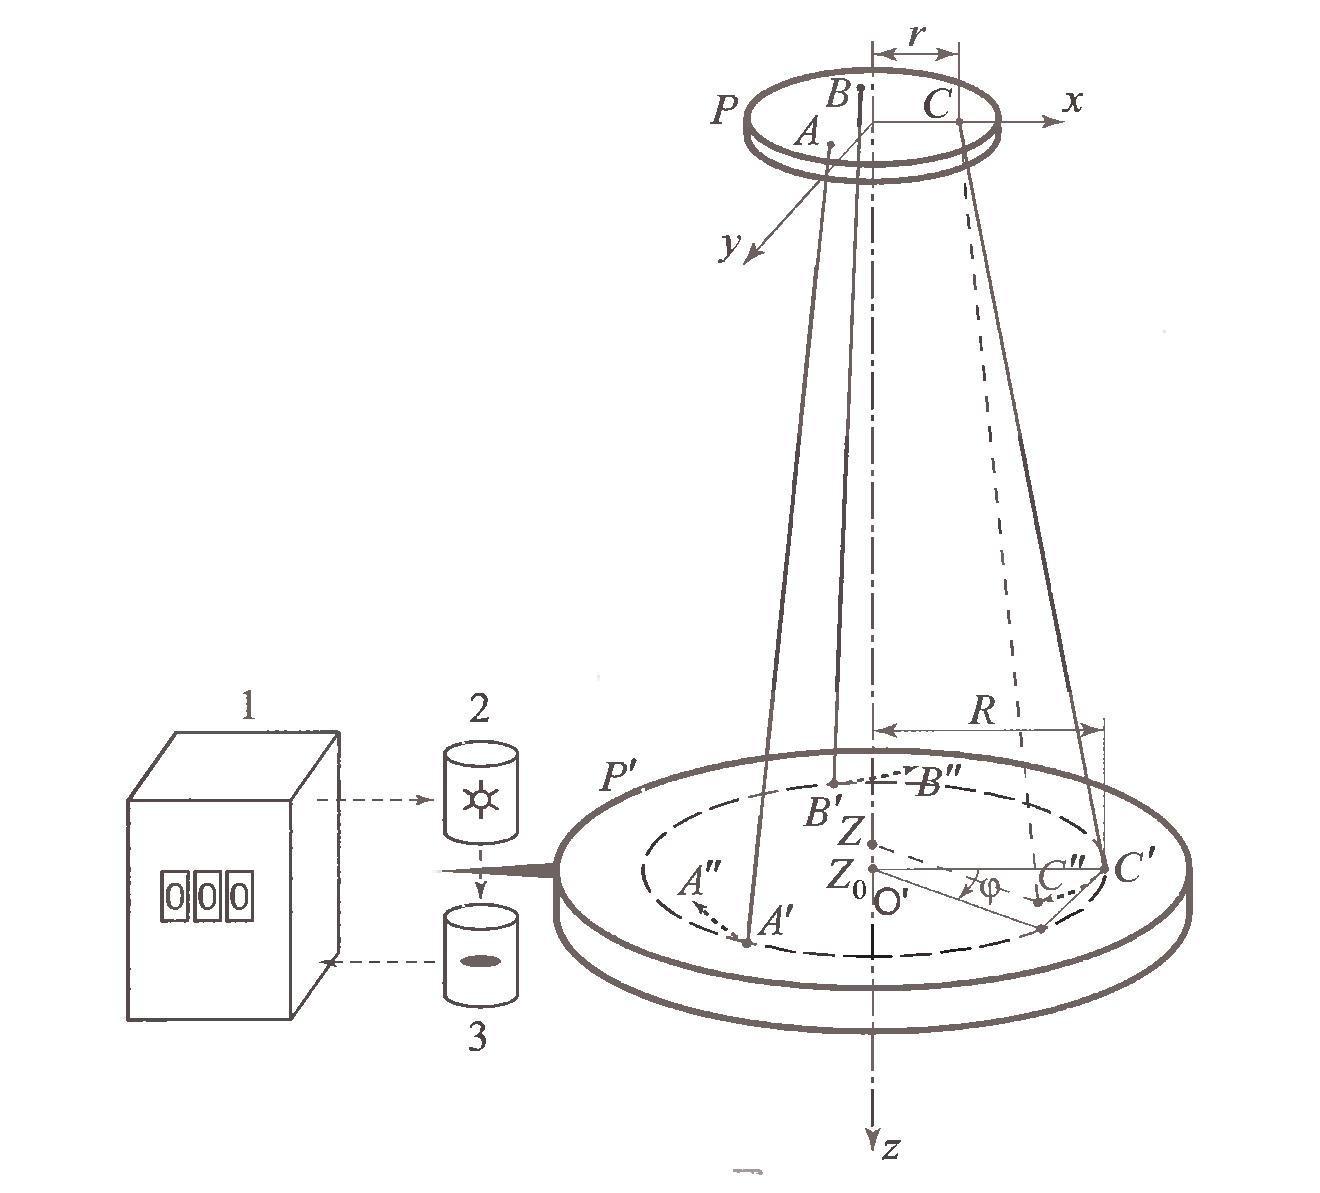
\includegraphics[width=1\linewidth]{1.2.3 ustan.jpg}
    \caption{Схема установки}
\end{minipage} \\
Учитывая, что при малых углах поворота $cos(\phi) \approx 1 - \frac{\phi^2}{2}$
\begin{center}
    $z \approx \sqrt{z_0 - Rr\phi^2} \approx z_0\sqrt{1-\frac{Rr\phi^2} {z_0^2}} \approx z_0 - \frac{Rr\phi^2}{2z_0}$
\end{center}
Подставляем это значение z в уравнение (2), получаем
\begin{center}
     $\frac{I {\dot{\phi}}^2}{2} + mg\frac{Rr}{z_0}\phi = E$
\end{center}
Решение этого уравнения колебаний имеет вид:
\begin{center}
     $\phi = \phi_0 sin\left(\sqrt{\frac{mgRr}{Iz_0}} + \Omega\right)$,
\end{center}
Период крутильных колебани нашей системы равен 
\begin{center}
    $T = 2\pi\sqrt{\frac{Iz_0}{mgRr}}$
\end{center}
Тогда формула для определения момента инерции:
\begin{center}
    $I = \frac{mgRrT^2}{4 \pi^2 z_0}$
\end{center}

\section{Оборудование и инструментальные погрешности}
\textit{В работе используются:} трифилярный подвес, секундомер, счетчик числа колебаний, набор тел, момент инерции которых надлежит измерить (диск, стержень, полый цилиндр и другие), линейка, штангенциркуль. \\
\textbf{Линейка:} $\delta_{lin} \pm 0.5$ мм \\
\textbf{Штангенциркуль:} $\delta_{tram} \pm 0.5$ мм (маркировка производителя)
\section{Результаты измерений и обработка данных}

Координата по вертикали центра нижней платформы $O^\prime$ при равновесии ($\phi$ = 0) $z_0 = 215$ см \\
Расстояние от центра малого диска до точки крепления нити: $r = (30 \pm 0.3)$ мм\\
Расстояние от центра малого диска до точки крепления нити: $R = (114.6 \pm 0.5)$ мм\\
Константа установки: $k = \frac{gRr}{4 \pi^2 z_0} \approx 4.05 \cdot 10^{-4}$ м$^2/c^2$ \\
Абсолютная погрешность: $\delta_k = k \cdot \sqrt{\left(\frac{\delta}{z_0}\right)^2 + \left(\frac{\delta}{R}\right)^2 + \left(\frac{\delta}{r}\right)^2 } \approx 0.07 \cdot 10^{-4}$ м$^2/c^2$
\subsection{Определение момента инерции ненагруженной платформы}
Масса платформы: M = $965.7 \pm 0.5$\\
Время колебаний: $\tau = 61~c$ \\ 
Кол-во обращений: N = 11\\
Период колебаний T = $4.36~c$\\
$\Rightarrow$ Момент инерции платформы: $I = 0.007$ кг $\cdot$ м$^2$
\subsection{Определение момента инерции тел}
\subsubsection{Согласно экспериментальным данным}
Относительная погрешность определения момента инерции: $\epsilon_I = \epsilon_T+\epsilon_k = 0.5\% + \frac{\delta_k}{k}\cdot100\% = 0.5\% + 2\% = 2.5\%$
Заполняем \textit{таблицу 1}

\begin{center}
\caption{Таблица № 1} \\
\begin{tabular}{| c | c | c | c | c | c | c |}

\hline
№ & Название &m,~г & \tau,~c & N & T,~c & I, $10^{-3}$ кг $\cdot$ м $^2$\\
\hline
1 & Брусок        & 1100.9 & 36.54 & 10 & 4.36 & 4.22\\
\hline
2 & Диск с пипкой & 881.3  & 36.97 & 10 & 4.45 & 2.74\\
\hline
3 & Цилиндр       & 730.3  & 49.74 & 12 &  4.14 & 4.79\\ 
\hline
\end{tabular}
\end{center}
m - масса тела (без платформы), $\tau$ - время вращения тела с платформой, N - кол-во оборотов, T - период колебаний, I - момент инерции тела.\\

Поставим 1ое и 2ое тела на платформу вместе, так чтобы центр масс системы оставался в центре диска. Посчитаем суммарный момент инерции этих тел:
cуммарная масса $m_{\Sigma} = m_1 + m_2 = 1982.2$ г, $\tau = 39.52$ с, $N = 10$ $\Rightarrow T = 3.952 \Rightarrow I = 6.64 \cdot 10^{-3}$ кг $\cdot$ м $^2$
Видно, что $I_{\Sigma} \approx I_1 + I_2 = 6.78$ кг $\cdot$ м$^2$ $\Rightarrow$ \textbf{\textit{аддитивность моментов инерции выполняется}}.
\subsubsection{Согласно теоретическим данным}
\begin{itemize}
    \item \textbf{Брусок} \\
        Длина $a = 21$ см \\
        Ширина $b = 2.6$ см \\
        Масса бруска m = 1100.9 г \\
        Момент инерции вдоль оси OZ: $I_z = \frac{m}{12}(a^2 + b^2) = 4.1\cdot10^{-3}$ кг$\cdot$м$^2$
    \item \textbf{Диск с пипкой} \\
        Больший диаметр $D = 16.1$ см \\
        Меньший диаметр $d = 2$ см \\
        Общая масса конструкции $m = 881.3$ г \\
        Высота большого основания $h_D = 0.5$ см\\
        Высота пипки $h_d = 1.5$ см \\
        Отношение масс $\frac{m_D}{m_d} = \frac{V_D}{V_d} = \frac{D^2 \cdot h_D}{d^2 \cdot h_d} \approx 21.6$ \Rightarrow Масса большего основания $m_D \approx 841.3$ г, а масса пипки $m_d \approx 40 $ г \\
        Момент инерции вдоль оси OZ: $I_z = \frac{m_D D^2}{8} + \frac{m_d d^2}{8} = 2.73 \cdot 10^{-3}$ кг$\cdot$м$^2$
    \item \textbf{Цилиндр} \\
        Диаметр кольца $d = 15.9$ см\\
        Масса цилиндра m = 730.3 г \\
        Момент инерции вдоль оси OZ: $I_z = \frac{md^2}{4} = 4.6 \cdot 10^{-3}$ кг$\cdot$м$^2$
    
\end{itemize}

\section{Нахождение массы и момента инерции однородного полного цилиндра}
Поместим на платформу шайбу, разрезанную по диаметру. Когда мы раздвигаем половинки выполняется теорема Штейнера. А именно момент инерции выражается в каждом конкретном случае
\begin{center}
$I = I_{disk} + I^{h = 0}_{puck} + mh^2$ ,  
\end{center}
где $I_{disk}$ - момент инерции диска (опоры), $I^{h = 0}_{puck}$ - момент инерции полной (без сдвига) шайбы. \\

Снимем зависимость момента инерции I такой 
системы от расстояния h между центром одной из половинок и центром платформы.\\
Масса системы: $M_{\Sigma} = 2501.6$ кг\\
Момент инерции $I = k \cdot M_{\Sigma} \cdot T^2$\\

\begin{minipage}[h]{0.5\linewidth}
Заполняем \textit{таблицу 2} \\
Строим график $I(h^2)$\\
Массу или коэффициент наклона графика можно посчитать как: 
\begin{center}
    $k = \frac{\langle I h^2 \rangle - \langle I \rangle \langle h^2 \rangle}{\langle (h^2)^2 \rangle - \langle h^2 \rangle^2} \approx 1.54 \Rightarrow$ \\
    Абсолютная погрешность коэфф. наклона $\delta_k = \frac{1}{\sqrt{n}} \sqrt{\frac{\langle I^2 \rangle - \langle I \rangle^2}{\langle h^4 \rangle - \langle h^2 \rangle^2} - k^2} = 0.03 $
\end{center}
Таким образом масса полной шайбы по графику $m^{graph}_{puck} = (1.54 \pm 0.03)$ кг, cогласно показаниям весов масса шайбы $m^{scales}_{puck} = 1536.1$ г Видно, что масса, определенная по графику с хорошей точность совпадает с массой, показанной весами.\\
По смещению графика по оси I можно определить момент инерции шайбы в "склеенном" виде, а именно 
\begin{center}
    $I^{h = 0}_{puck} = I(0) - I_{disk} = 0.0086 - 0.007 = 0.0016$ кг $\cdot$ м$^2$ \\
    Абсолютна погрешность $\delta_{I^{h = 0}_{puck}} = \delta_m \cdot \sqrt{\langle h^4 \rangle + \langle h^2 \rangle^2} \approx 0.005$ кг $\cdot$ м$^2$
\end{center}

Согласно теоретическим данным момент инерции шайбы $I_{puck} = 
\frac{m_{puck}\cdot d_{puck}^2}{8} \approx 0.0017$ кг $\cdot$ м$^2$ \\
Как видно \textit{\textbf{теорема Гюйгенса-Штейнера действительно выполняется.}}
\end{minipage}
\begin{minipage}[h]{0.5\textwidth}
    \begin{table}[h]
        \centering
        \caption{Таблица № 2} \\
        \begin{tabular}{| c | c | c | c | c | c |}
        \hline
        № & h,~см & \tau,~c & N & T,~c & I, кг $\cdot$ м^2\\
        \hline
        1 & 0 & 29.1 & 10 & 2.91 & 0.0086\\
        \hline
        2 & 1 & 30.13 & 10 & 3.013 & 0.0092\\
        \hline
        3 & 2 & 29.63 & 10 & 2.96 & 0.0089\\
        \hline
        4 & 3 & 31.41 & 10 & 3.14 & 0.01\\
        \hline
        5 & 3.5 & 32.34 & 10 & 3.23 & 0.0106\\
        \hline
        6 & 4 & 33.09 & 10 & 3.31 & 0.0111\\
        \hline
        7 & 4.5 & 34.13 & 10 & 3.41 & 0.0118\\
        \hline
        8 & 5 & 34.84 & 10 & 3.48 & 0.0123\\
        \hline
        9 & 5.5 & 36.64 & 10 & 3.66 & 0.0136\\
        \hline
        10 & 6 & 37.31 & 10 & 3.73 & 0.0141\\
        \hline
        \end{tabular}
    \end{table}
    \centering
	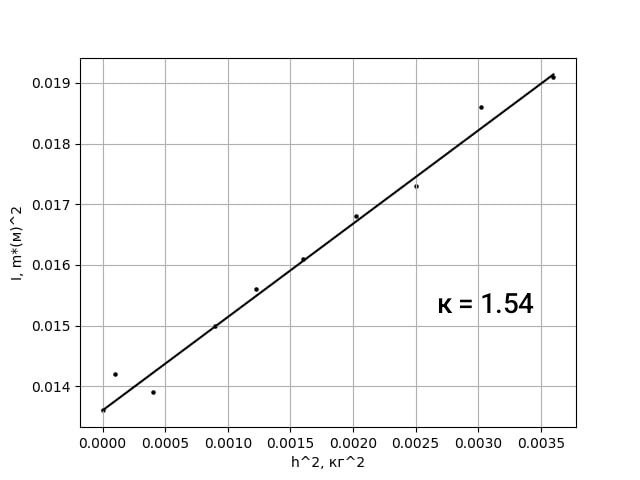
\includegraphics[width=1\linewidth]{Figure_2.png}
\end{minipage} \\
\section{Обсуждение результатов}
В данной работе были измерены моменты инерции нескольких тел теоретически и практически. С помощью трифилярного подвеса можно определять момент инерции с достаточно большой точностью $\varepsilon \approx 2.5\%$. Такая точность обусловлена малой погрешностью измерения времени и условиями, при которых колебания подвеса можно считать слабозатухающими. \\
\caption{Итоговая таблица} \\
\begin{tabular}{| c | c | c | c | c | c |}
\hline
Название & Рисунок & Момент инерции (на практике) & Момент инерции (в теории)\\
\hline
Брусок & 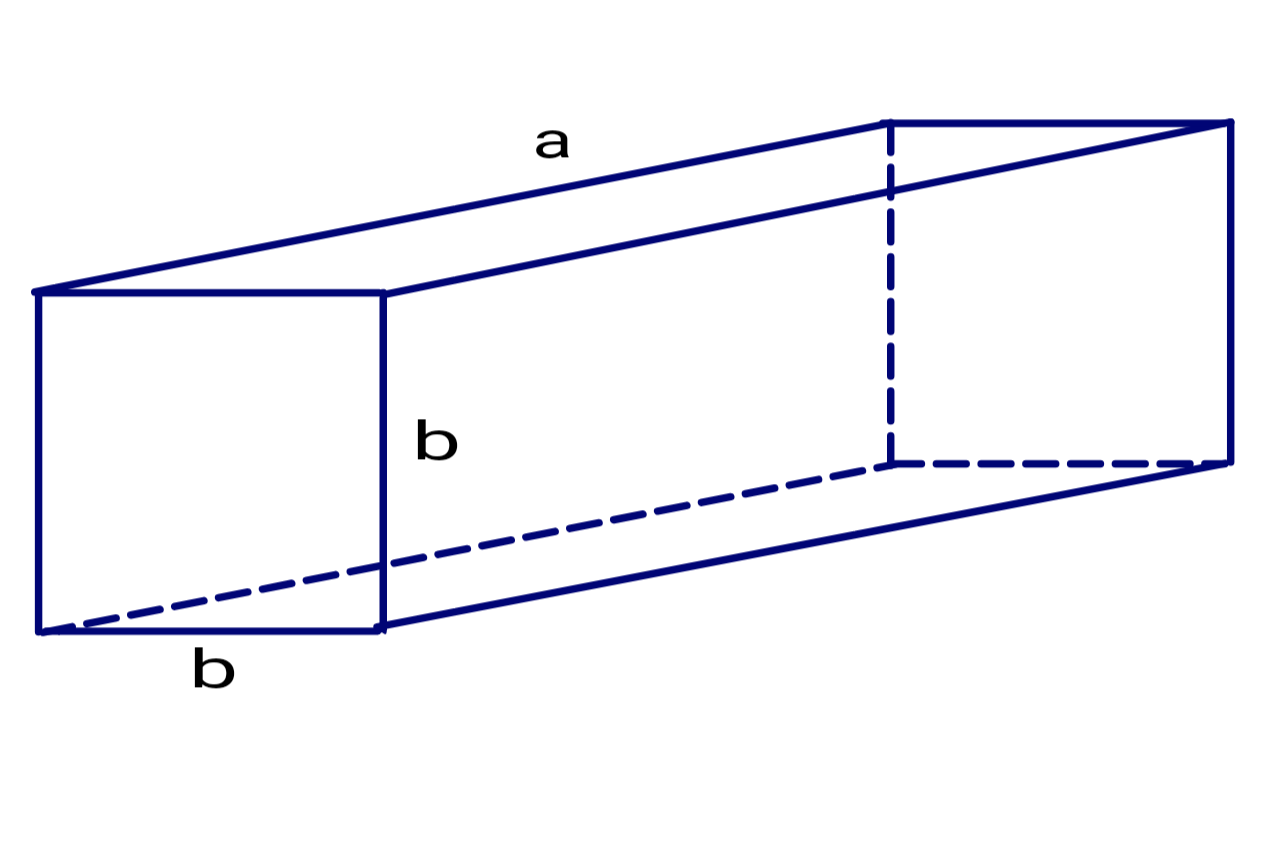
\includegraphics[scale=0.1]{kvadr.png} & 
(4.22 \pm~0.1) $ г\cdot$м^2 & 4.1 г $\cdot$ м^2\\
\hline
Диск с пипкой & 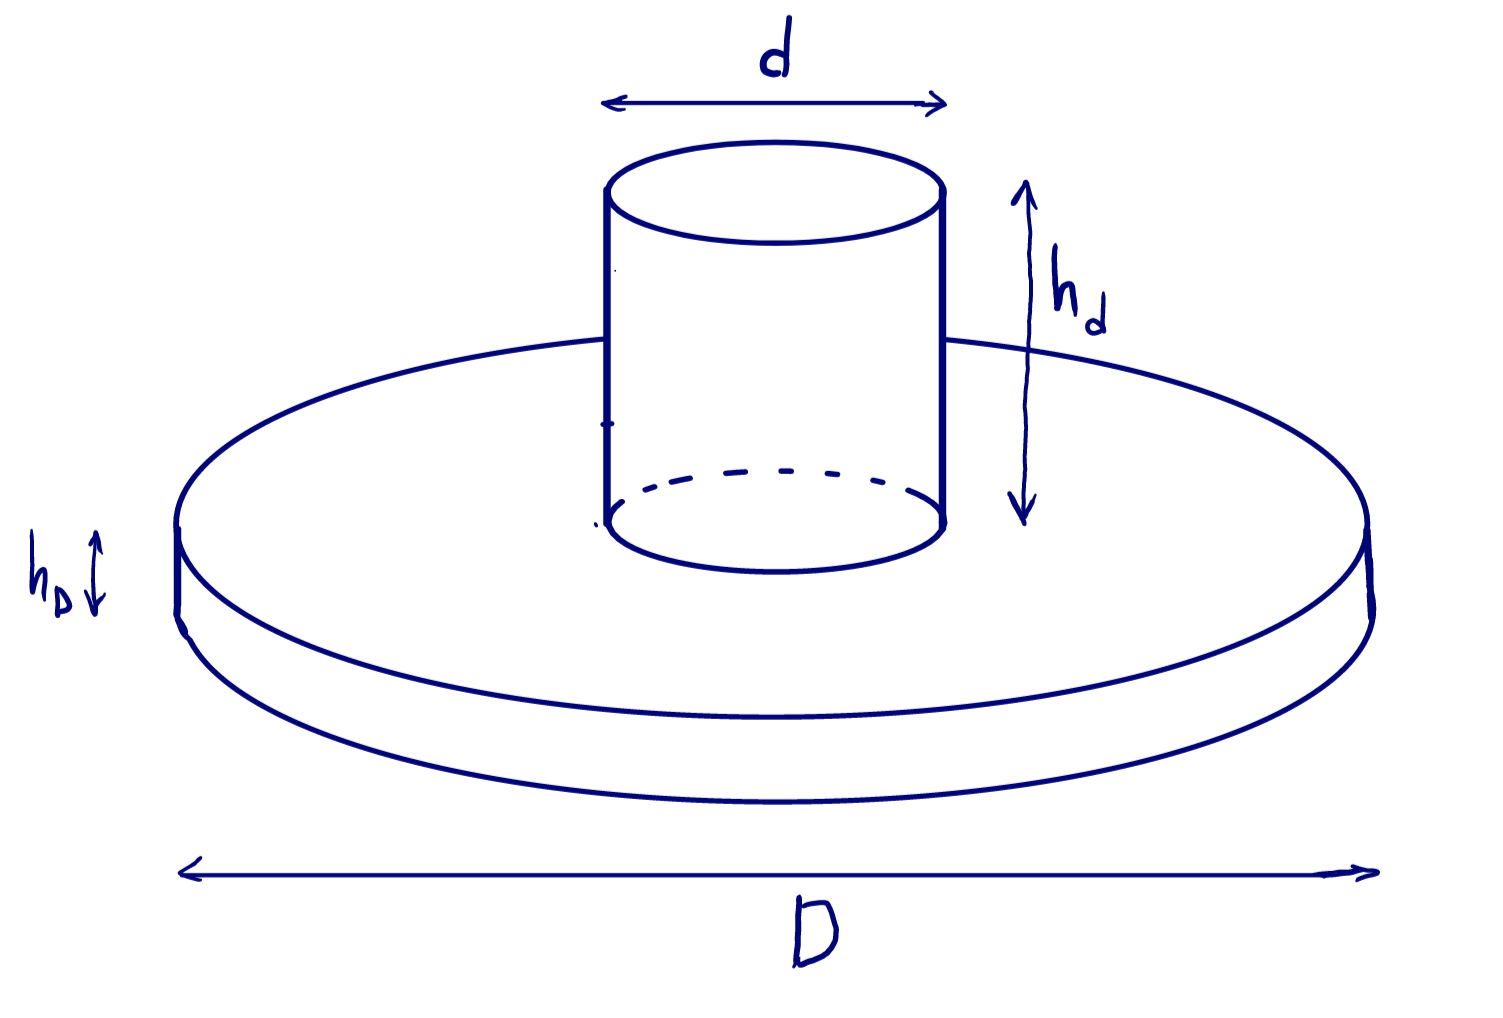
\includegraphics[scale=0.1]{cylinder+.png} & (2.74 \pm~0.07)$г\cdot$ м^2 & 2.73 г $\cdot$ м^2\\
\hline
Цилиндр & 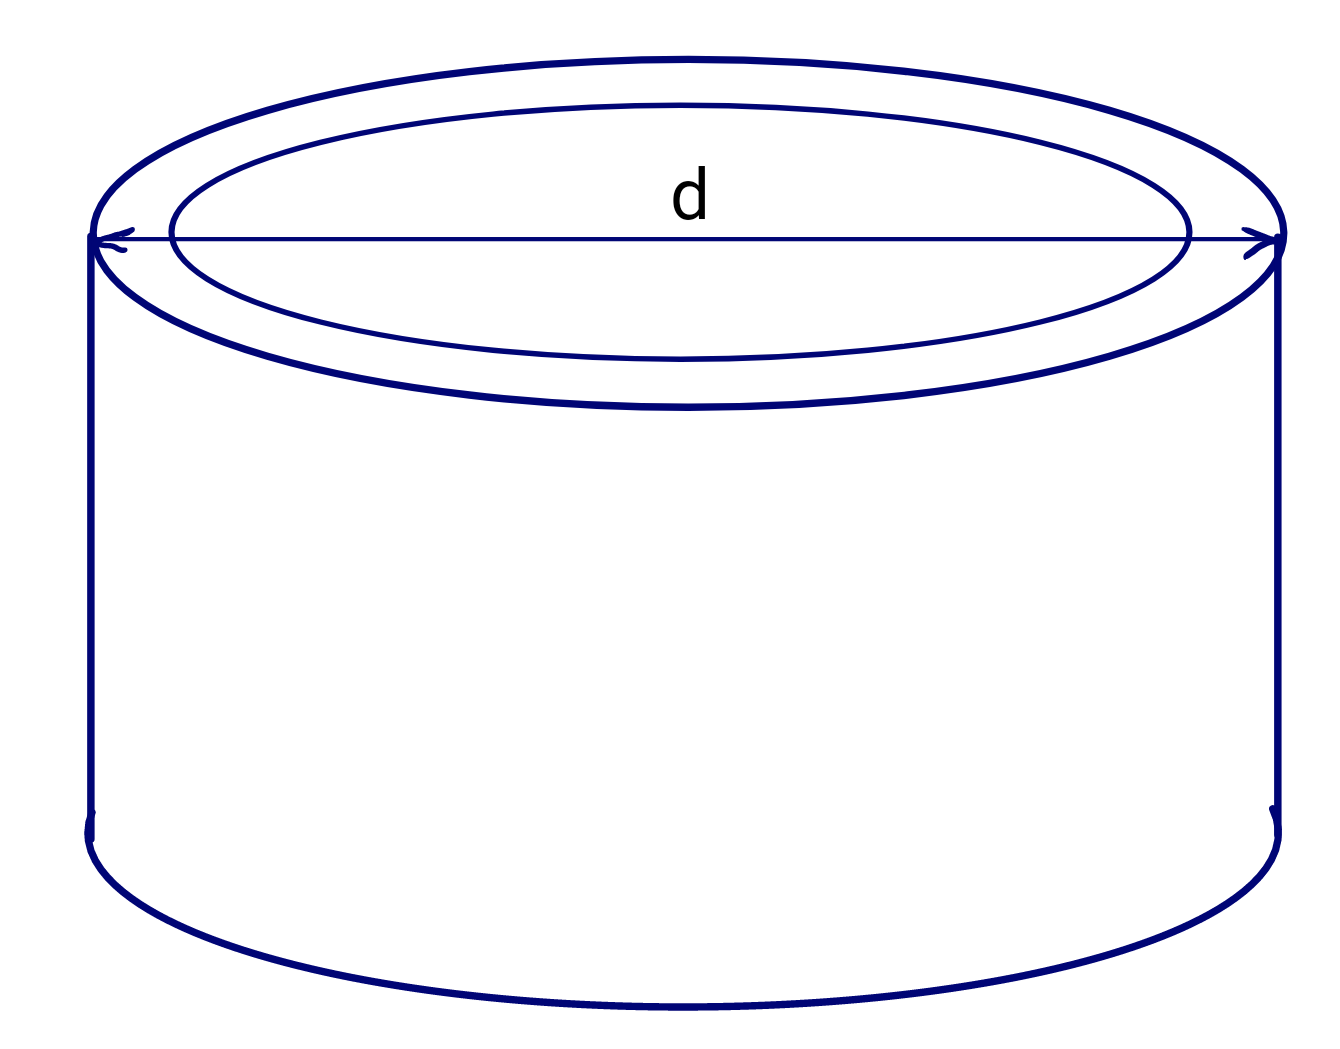
\includegraphics[scale=0.1]{cylinder.png}  & (4.79 \pm~0.12) г$\cdot$ м^2 & 4.6 г$\cdot$ м^2\\
\hline
\end{tabular}
В целом, значения момента инерции, полученные экспериментально и теоретически достаточно схожи. Большая погрешность исходит из подсчета коэффициента установки. Уменьшить её возможно, более точно измерив расстояния R и r, описанные в работе. \\
В работе показано, что выполняется аддитивность моментов инерции. Также показано, что выполняется теорема Гюйгенса-Штейнера.
\end{document}
